\documentclass{beamer}
\usetheme{Boadilla}

\usepackage{graphics}
\usepackage{float}

\title{Visualizasion of COVID-19 data, using pandas.}
%\subtitle{}
\author{Christian Berrig}
\institute{Roskilde Univarsity}
\date{\today}

\begin{document}

\begin{frame}
\titlepage
\end{frame}

\section{Raw data}
\subsection{Timeseries}

\begin{frame}
\frametitle{Timeseries: Cumulated numbers}
\begin{figure}[H]
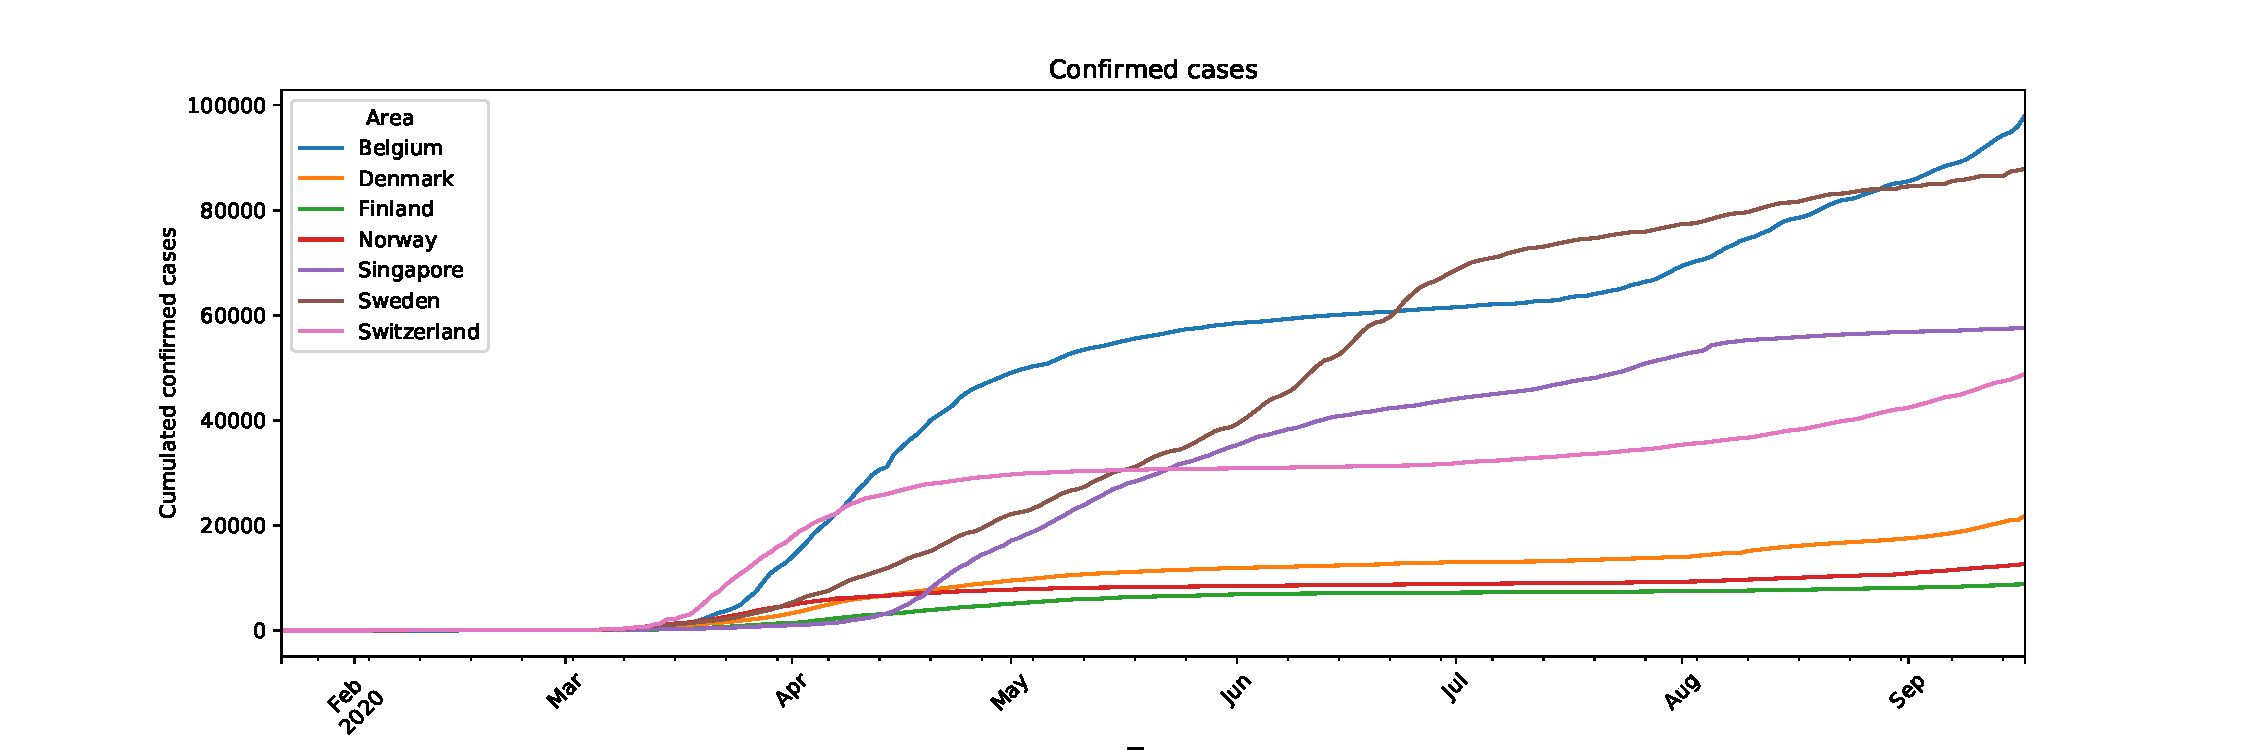
\includegraphics[width=\textwidth]{../figs/confirmed_timeseries_linear.pdf}
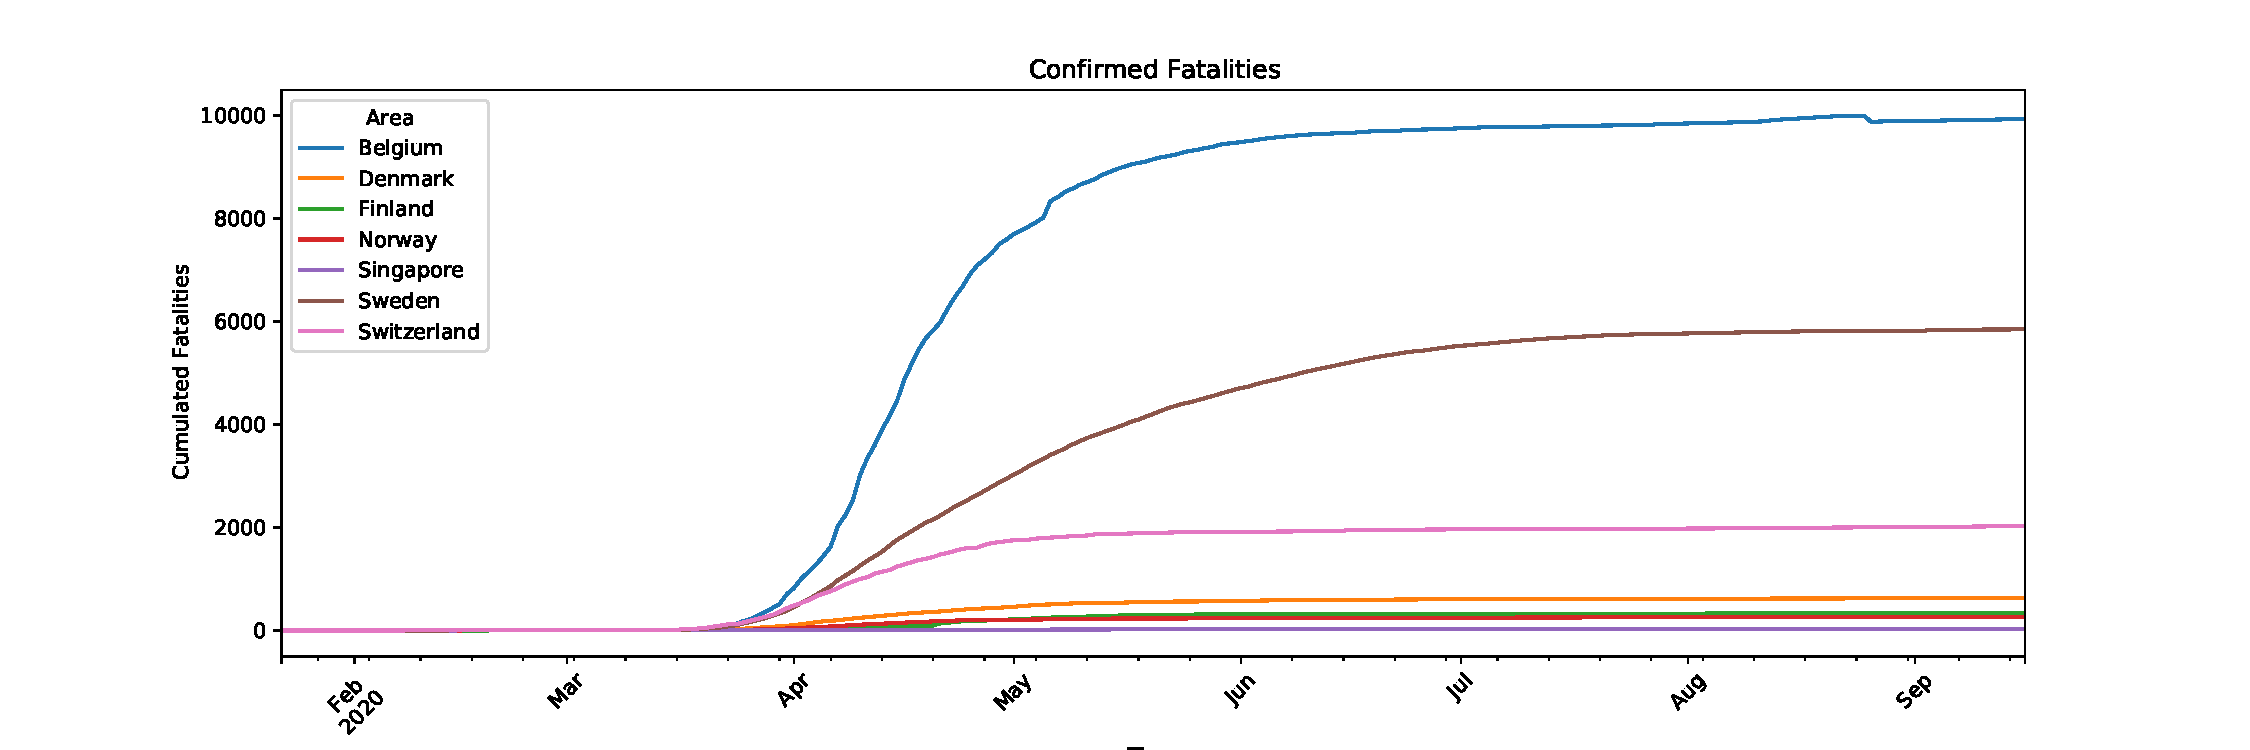
\includegraphics[width=\textwidth]{../figs/deaths_timeseries_linear.pdf}
\end{figure}
\end{frame}

\begin{frame}
\frametitle{Timeseries: generating the rates}
\begin{figure}[H]
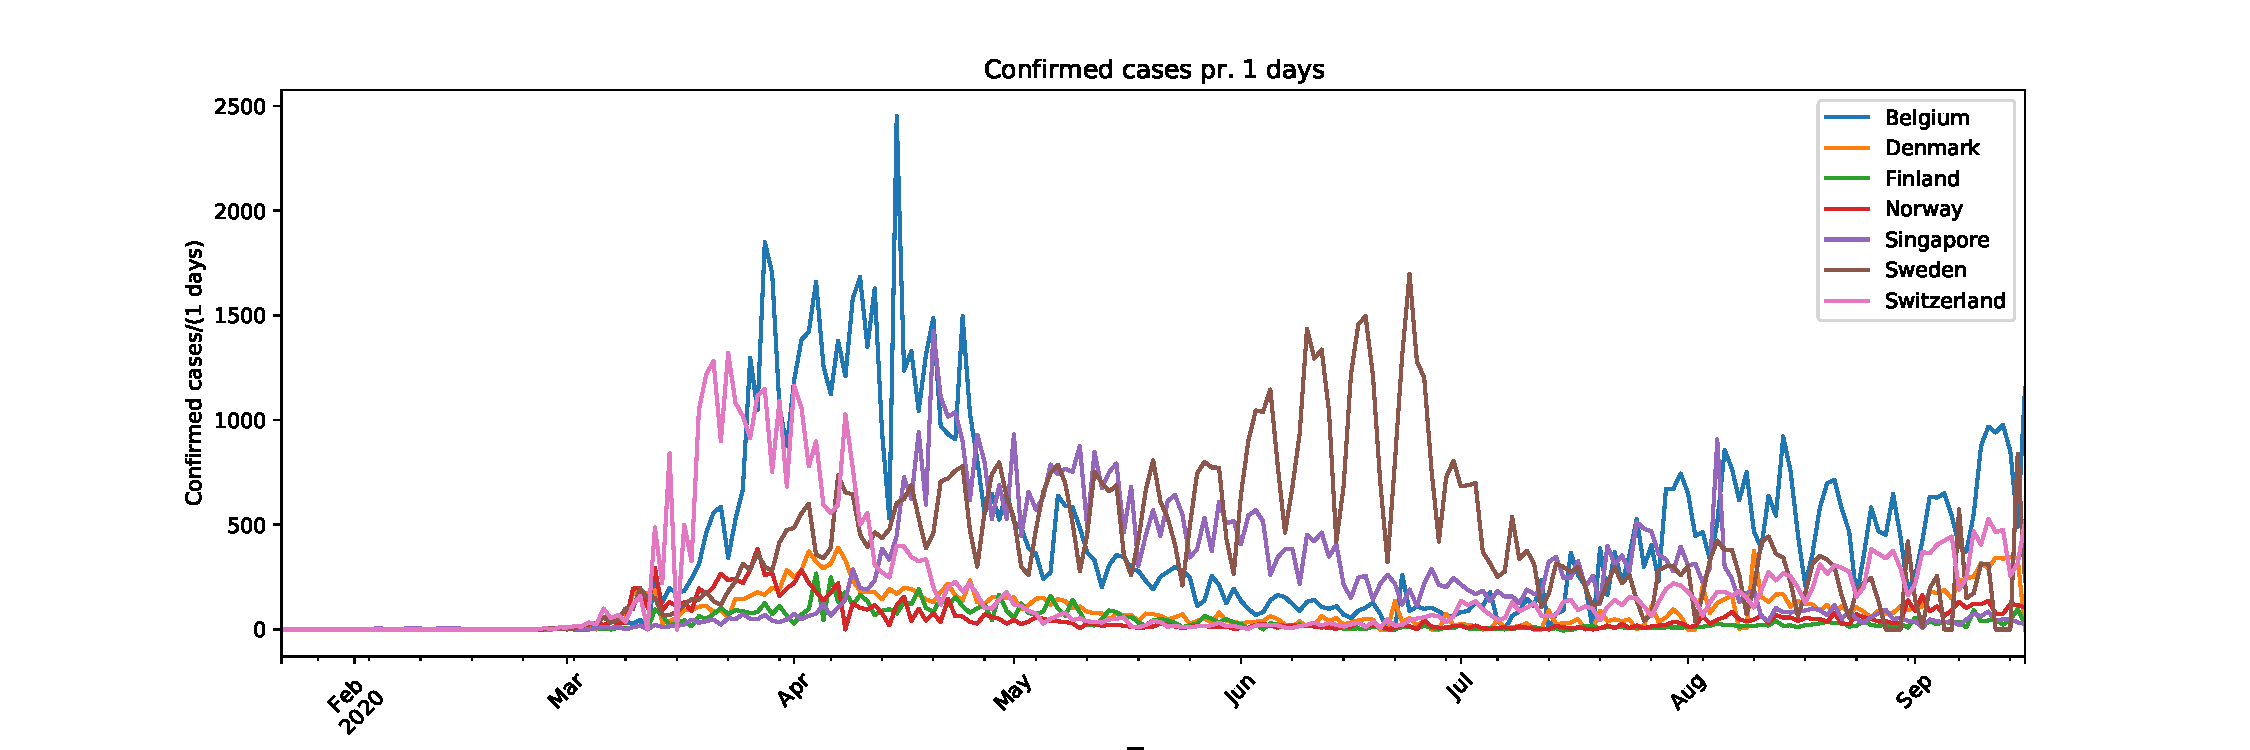
\includegraphics[width=\textwidth]{../figs/confirmed_rate_timeseries_1days_linear.pdf}
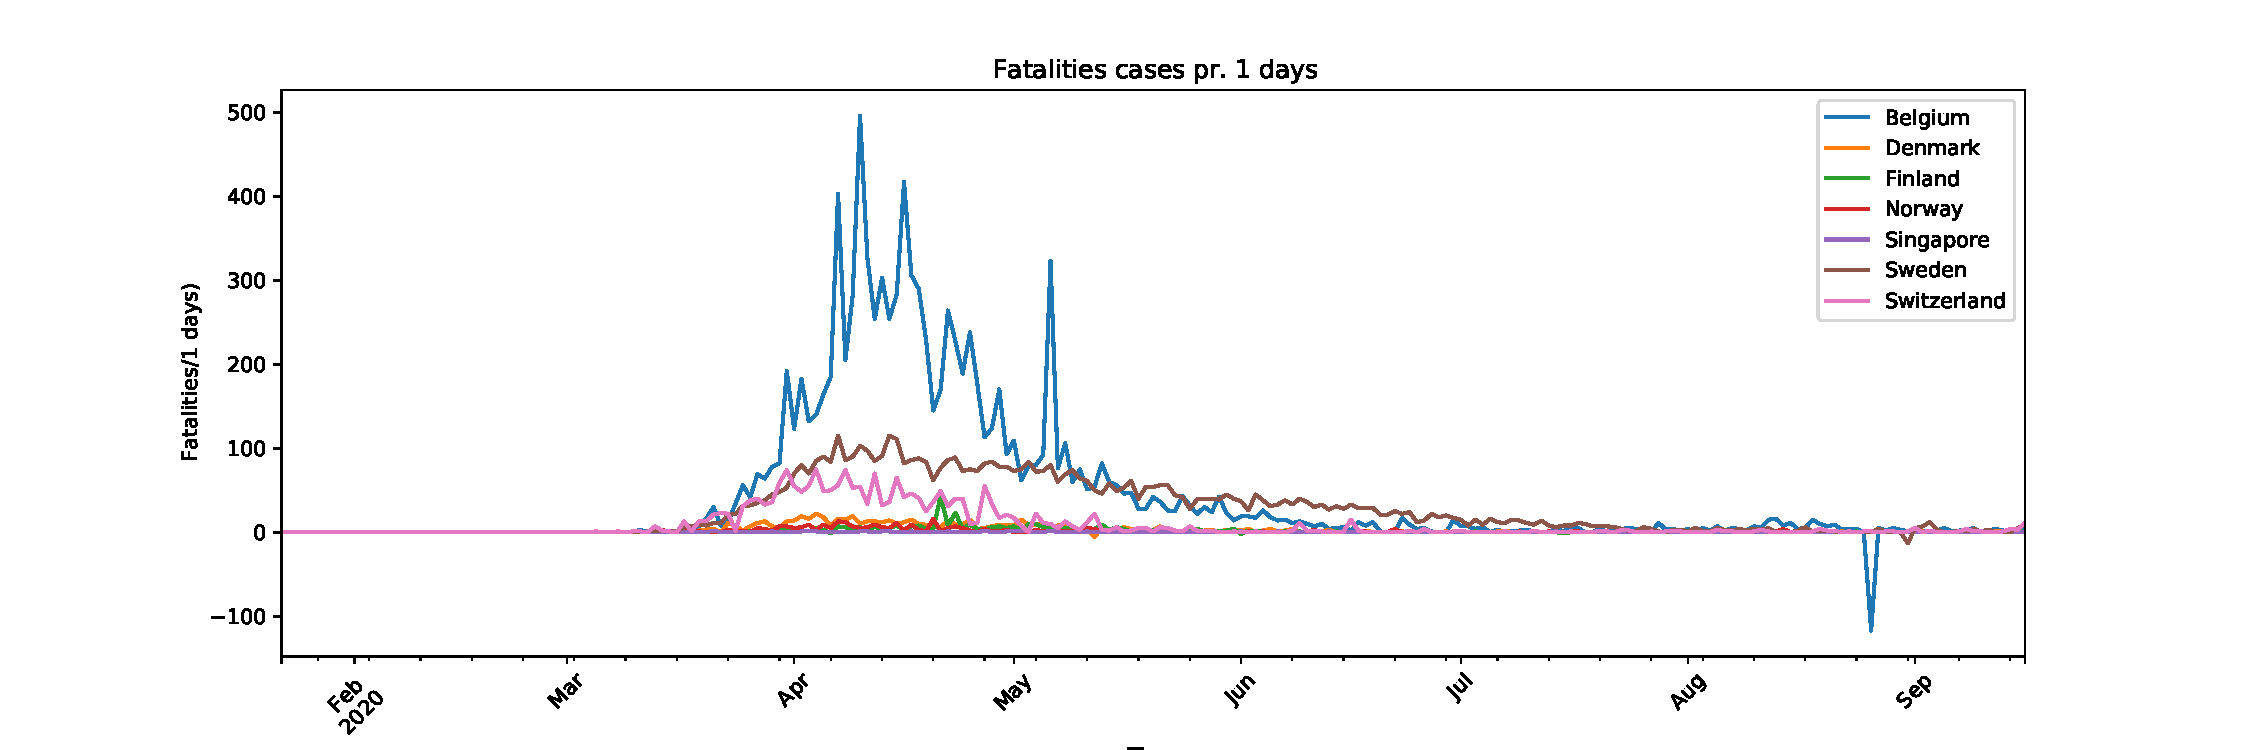
\includegraphics[width=\textwidth]{../figs/deaths_rate_timeseries_1days_linear.pdf}
\end{figure}
\end{frame}

\begin{frame}
\frametitle{Timeseries: generating the rates}
\begin{figure}[H]
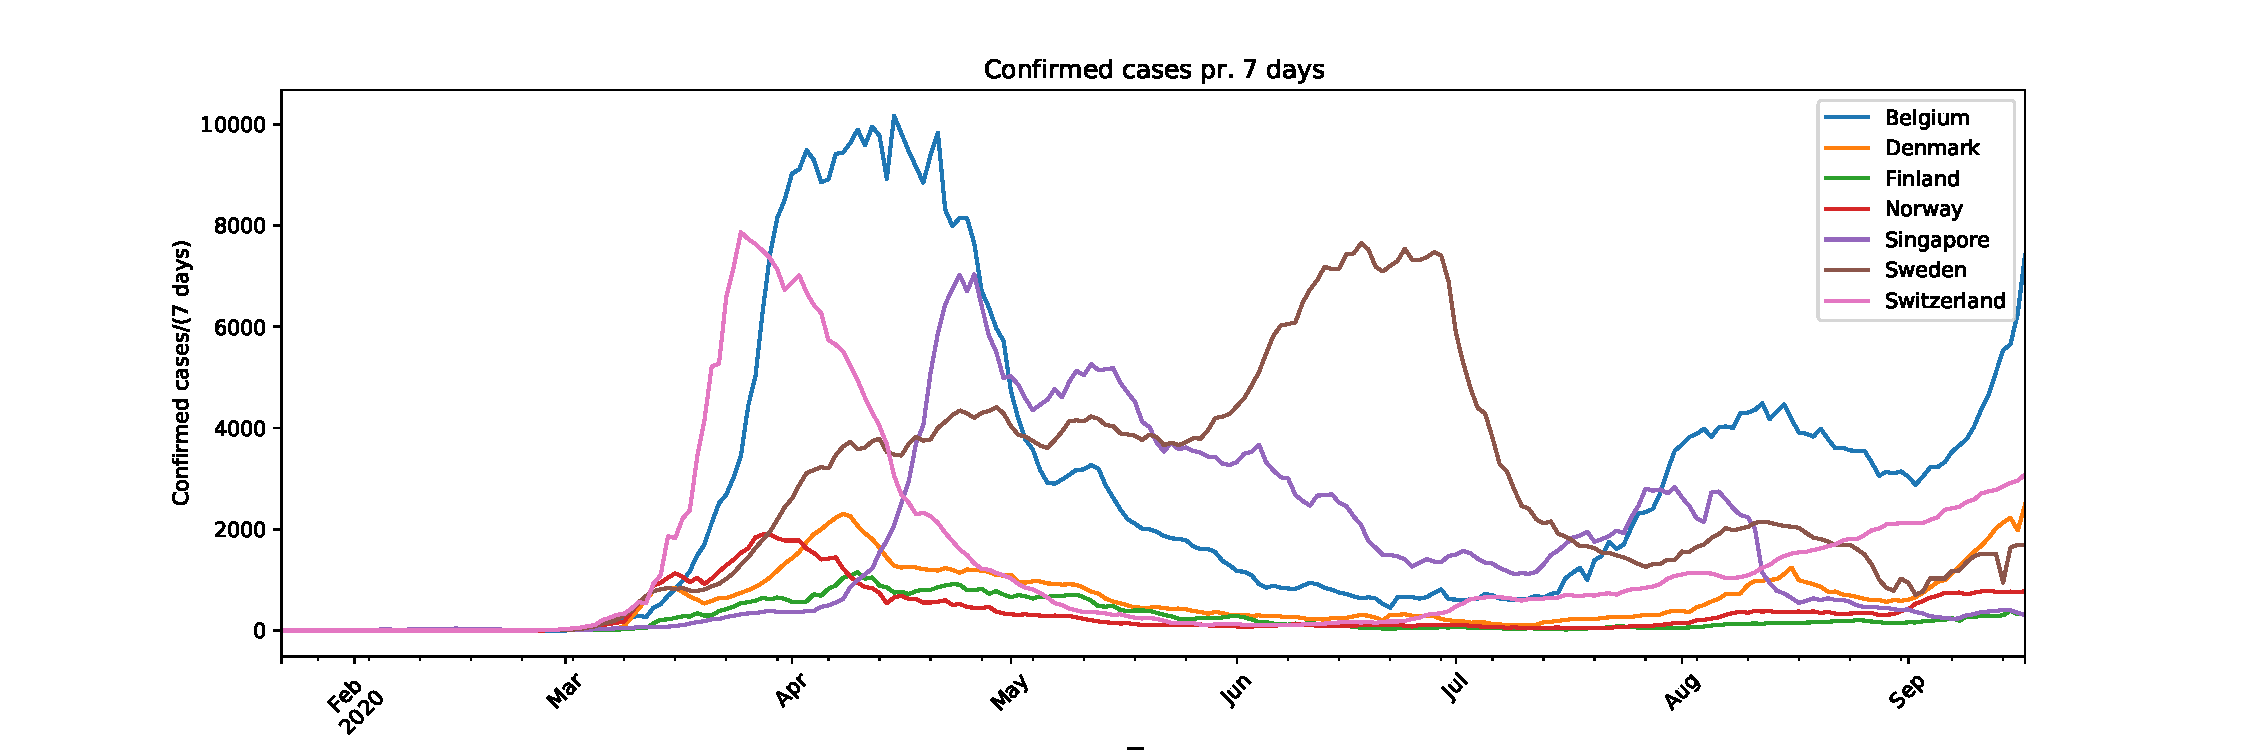
\includegraphics[width=\textwidth]{../figs/confirmed_rate_timeseries_7days_linear.pdf}
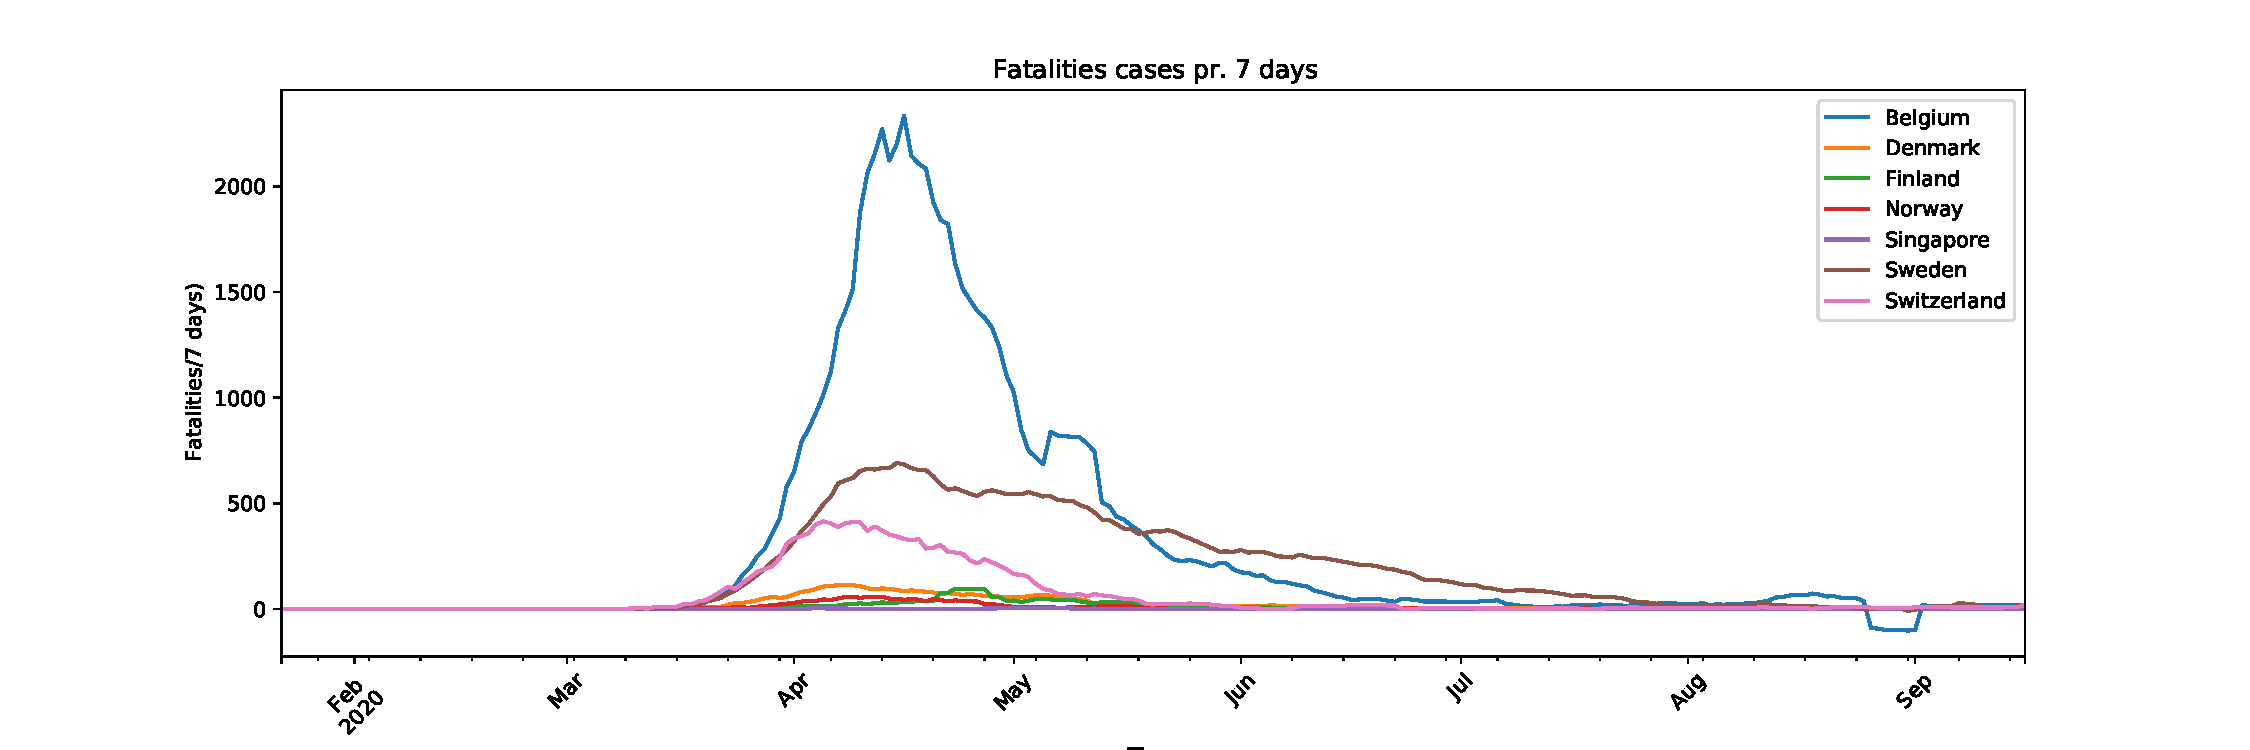
\includegraphics[width=\textwidth]{../figs/deaths_rate_timeseries_7days_linear.pdf}
\end{figure}
\end{frame}

\subsection{Parametric plot}
\begin{frame}
\frametitle{Parametric plots: raw numbers}
\begin{figure}[H]
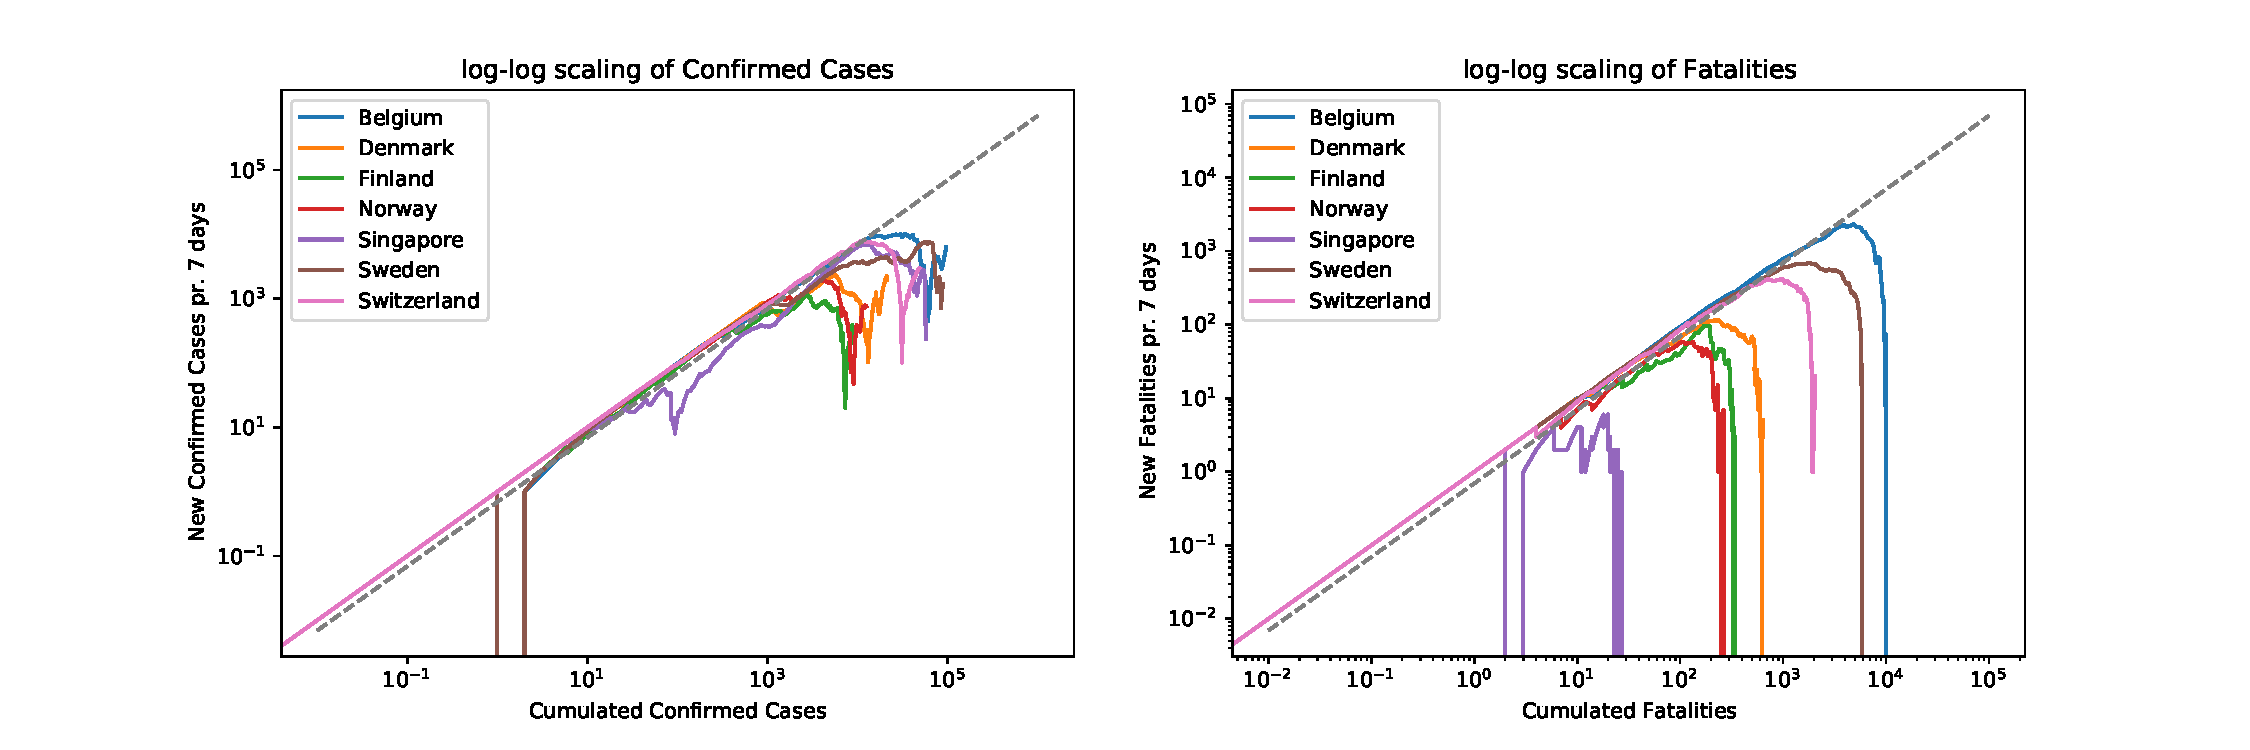
\includegraphics[width=\textwidth]{../figs/parametric_plots_log.pdf}
\end{figure}
\end{frame}

\section{Transformed data}
\subsection{Parametric plot: normalized and semi-normalized}
\begin{frame}
\frametitle{Parametric plots: normalized numbers}
\begin{figure}[H]
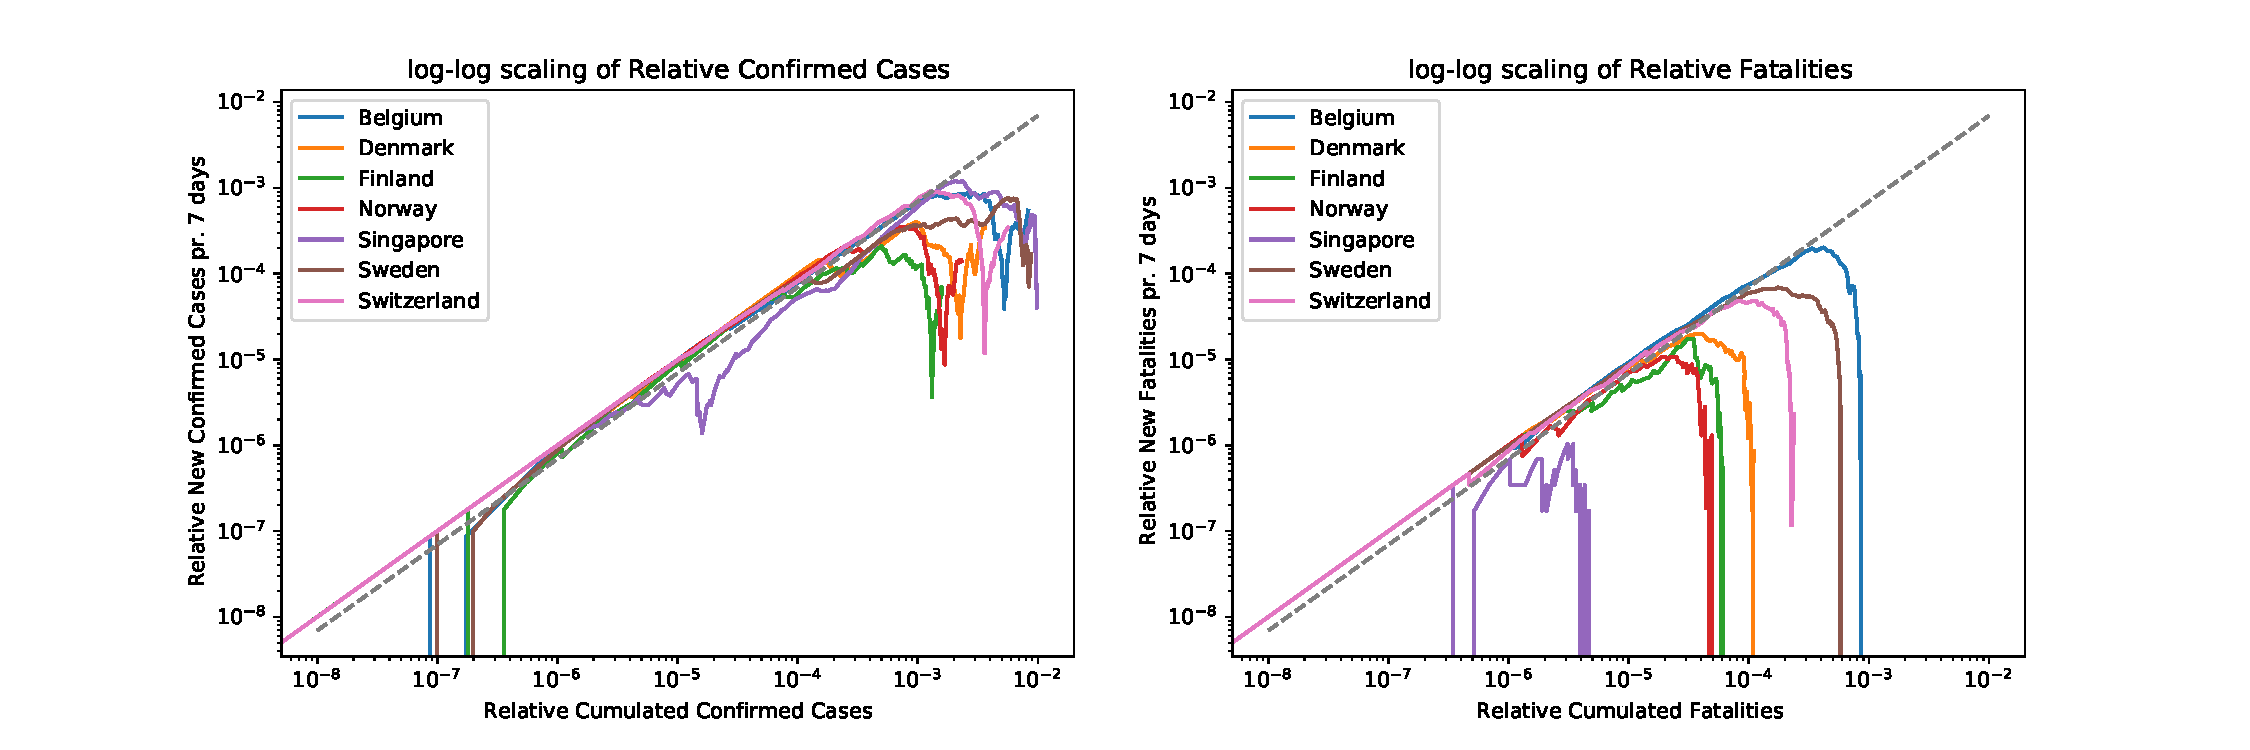
\includegraphics[width=\textwidth]{../figs/parametric_plots_normalized_log.pdf}
\end{figure}
\end{frame}

\begin{frame}
\frametitle{Parametric plots: semi-normalized}
\begin{figure}[H]
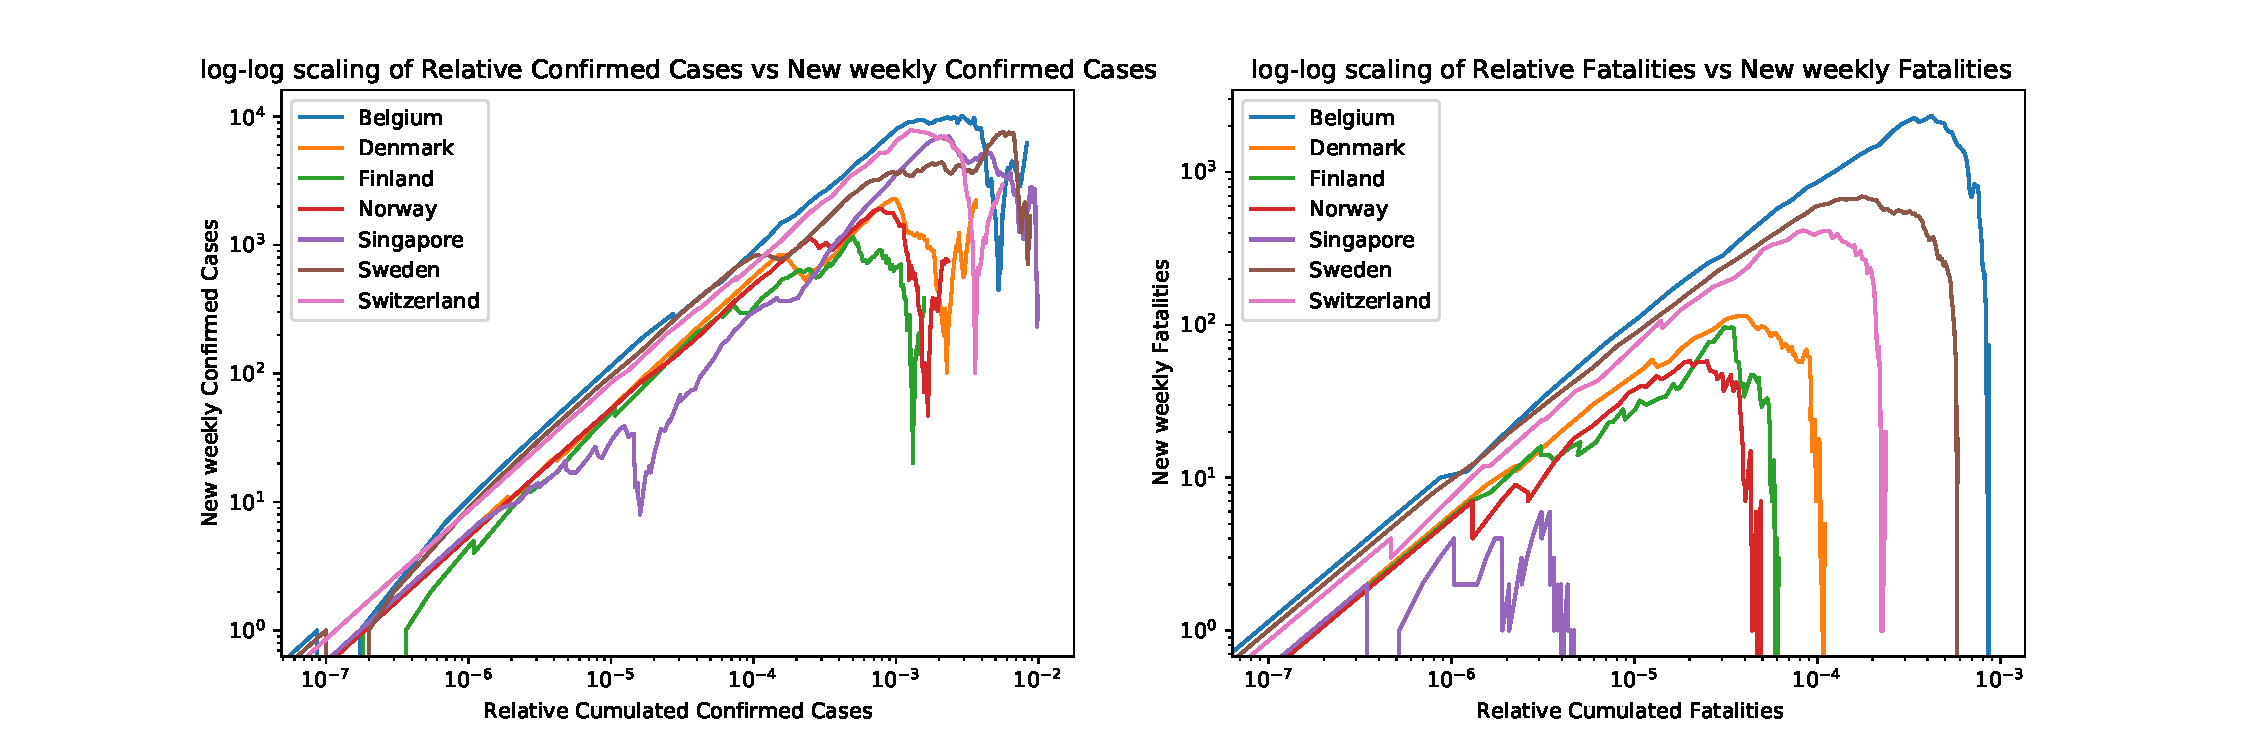
\includegraphics[width=\textwidth]{../figs/parametric_plots_semi-normalized_log.pdf}
\end{figure}
\end{frame}

\subsection{Timeseries: normalized data}
\begin{frame}
\frametitle{Timeseries: normalized numbers}
\begin{figure}[H]
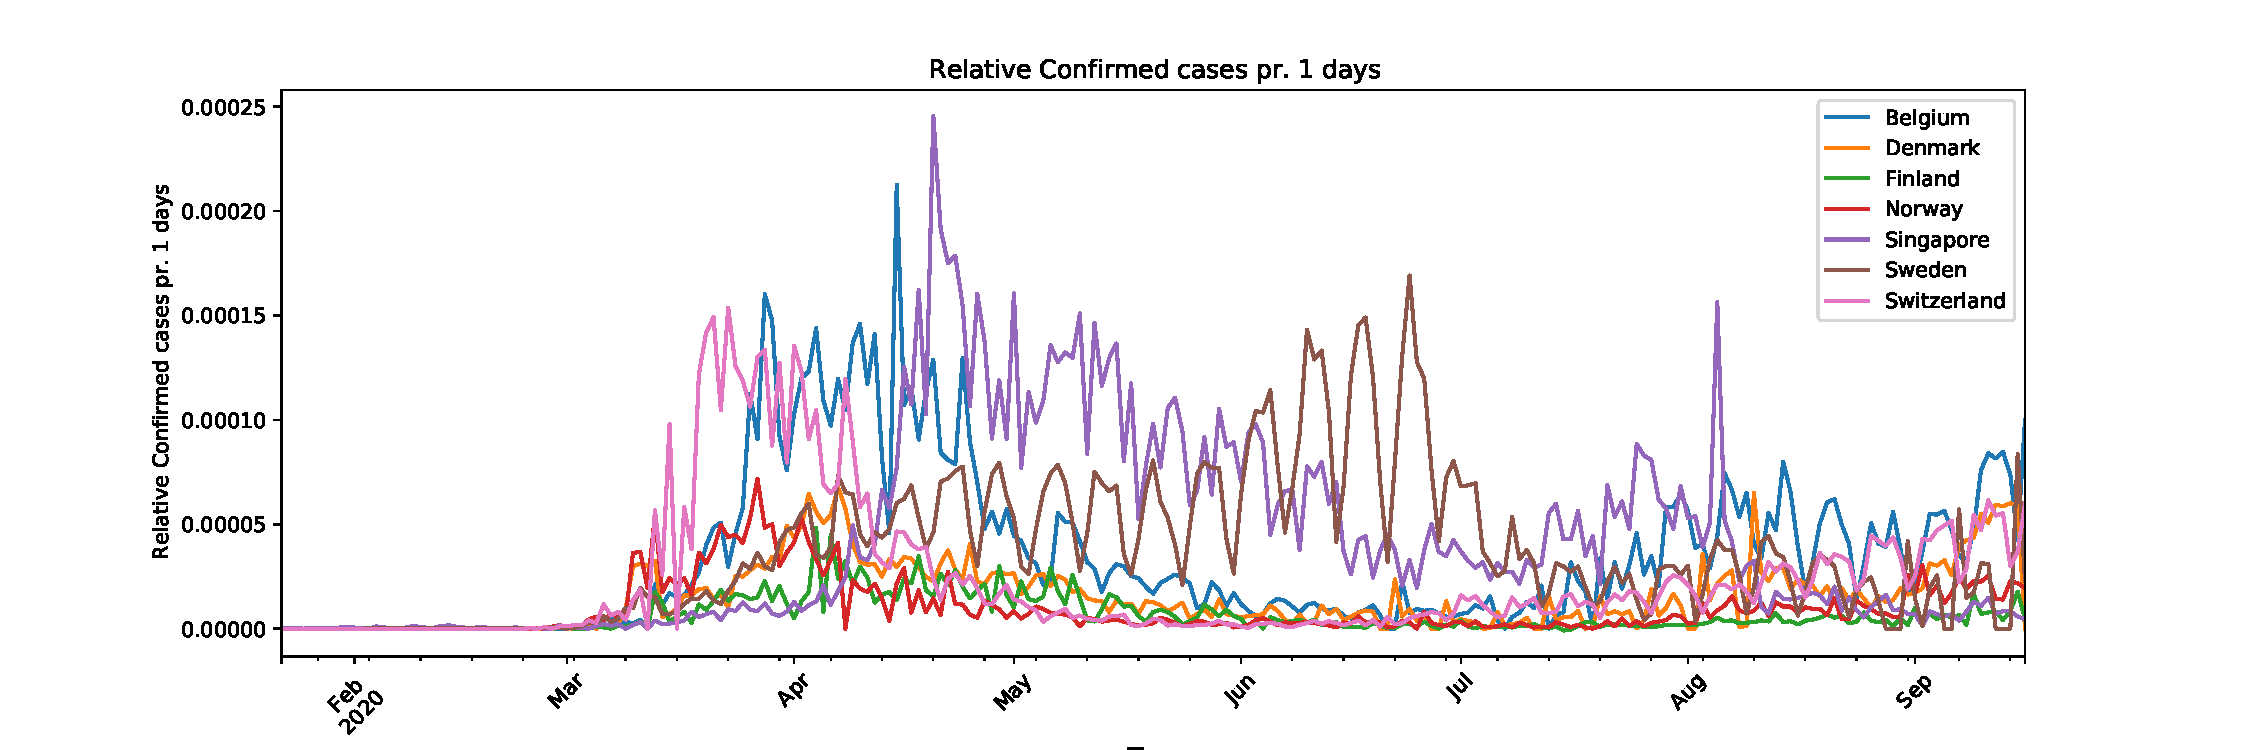
\includegraphics[width=\textwidth]{../figs/confirmed_rate_timeseries_relative_1days_linear.pdf}
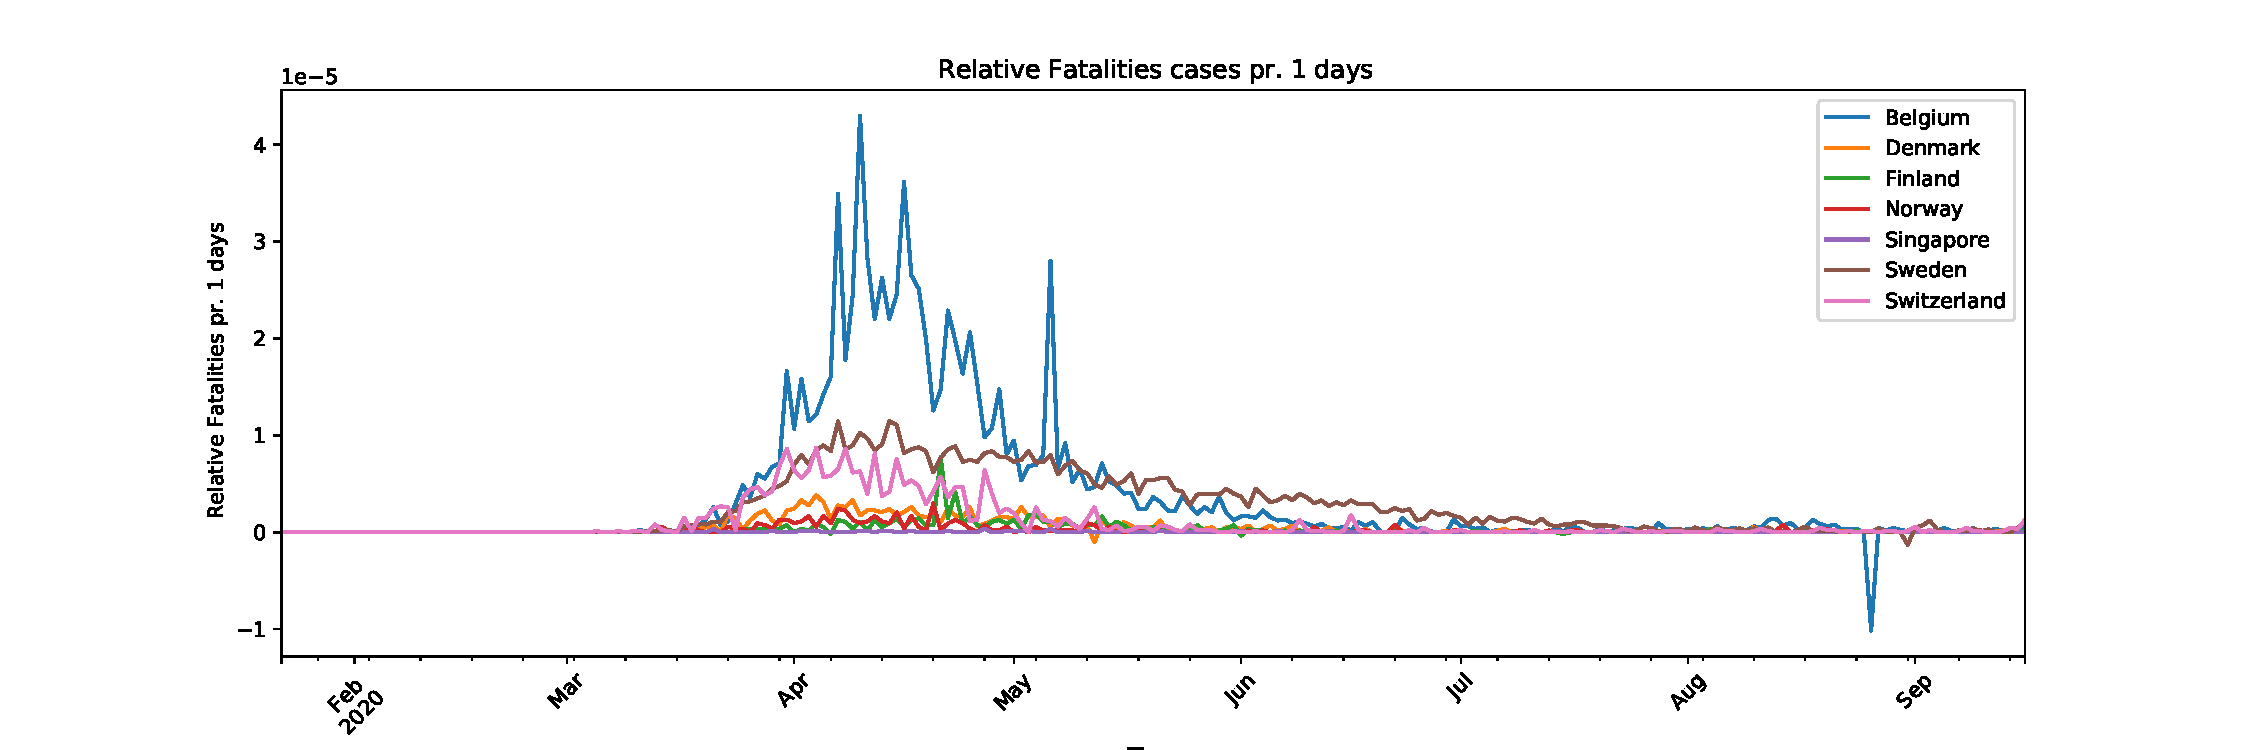
\includegraphics[width=\textwidth]{../figs/deaths_rate_timeseries_relative_1days_linear.pdf}
\end{figure}
\end{frame}
\begin{frame}
\frametitle{Timeseries: normalized numbers}
\begin{figure}[H]
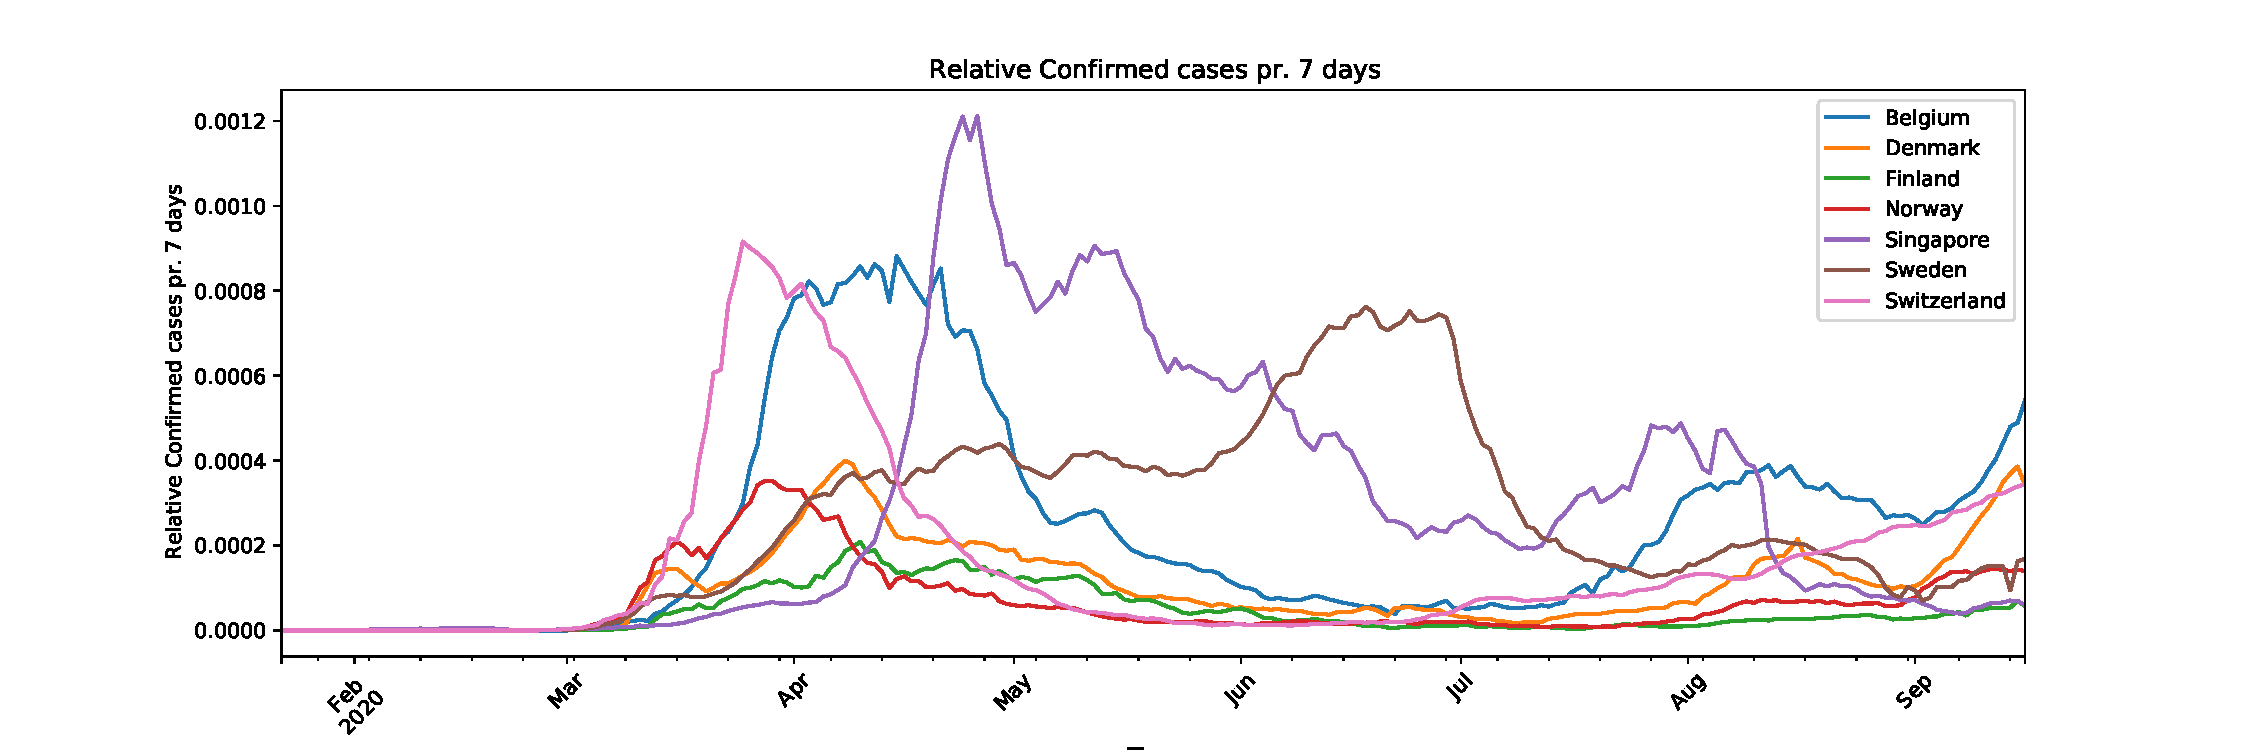
\includegraphics[width=\textwidth]{../figs/confirmed_rate_timeseries_relative_7days_linear.pdf}
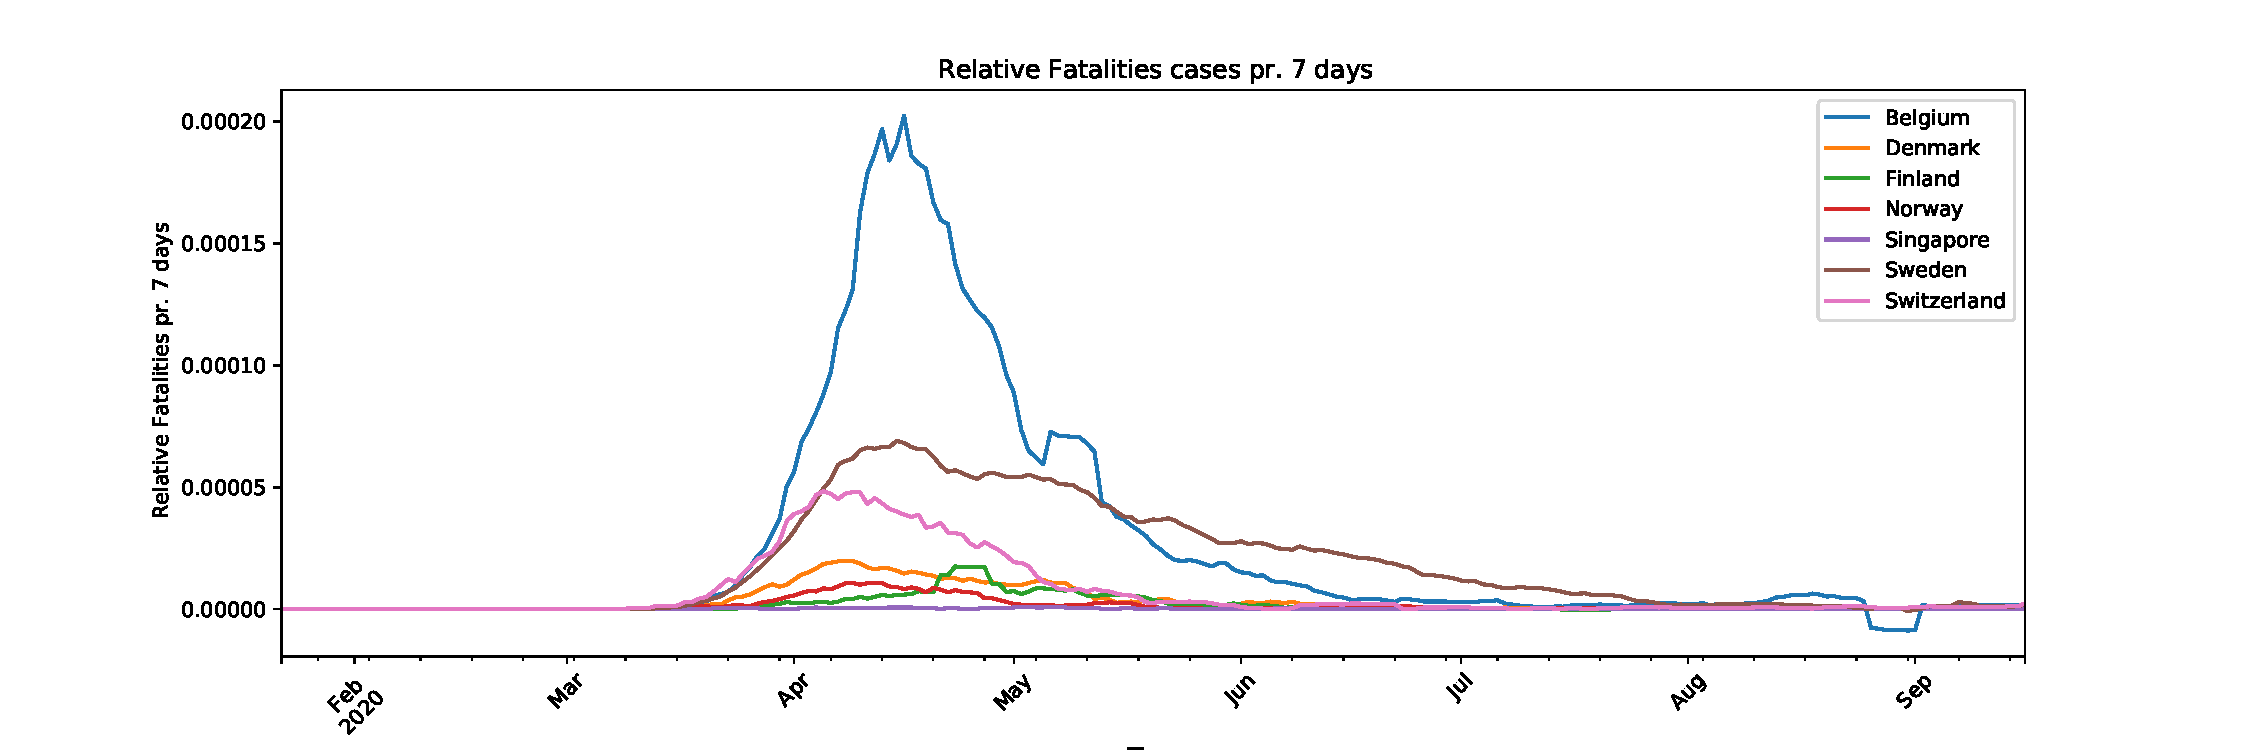
\includegraphics[width=\textwidth]{../figs/deaths_rate_timeseries_relative_7days_linear.pdf}
\end{figure}
\end{frame}

\begin{frame}
\frametitle{Timeseries: normalized numbers}
\begin{figure}[H]
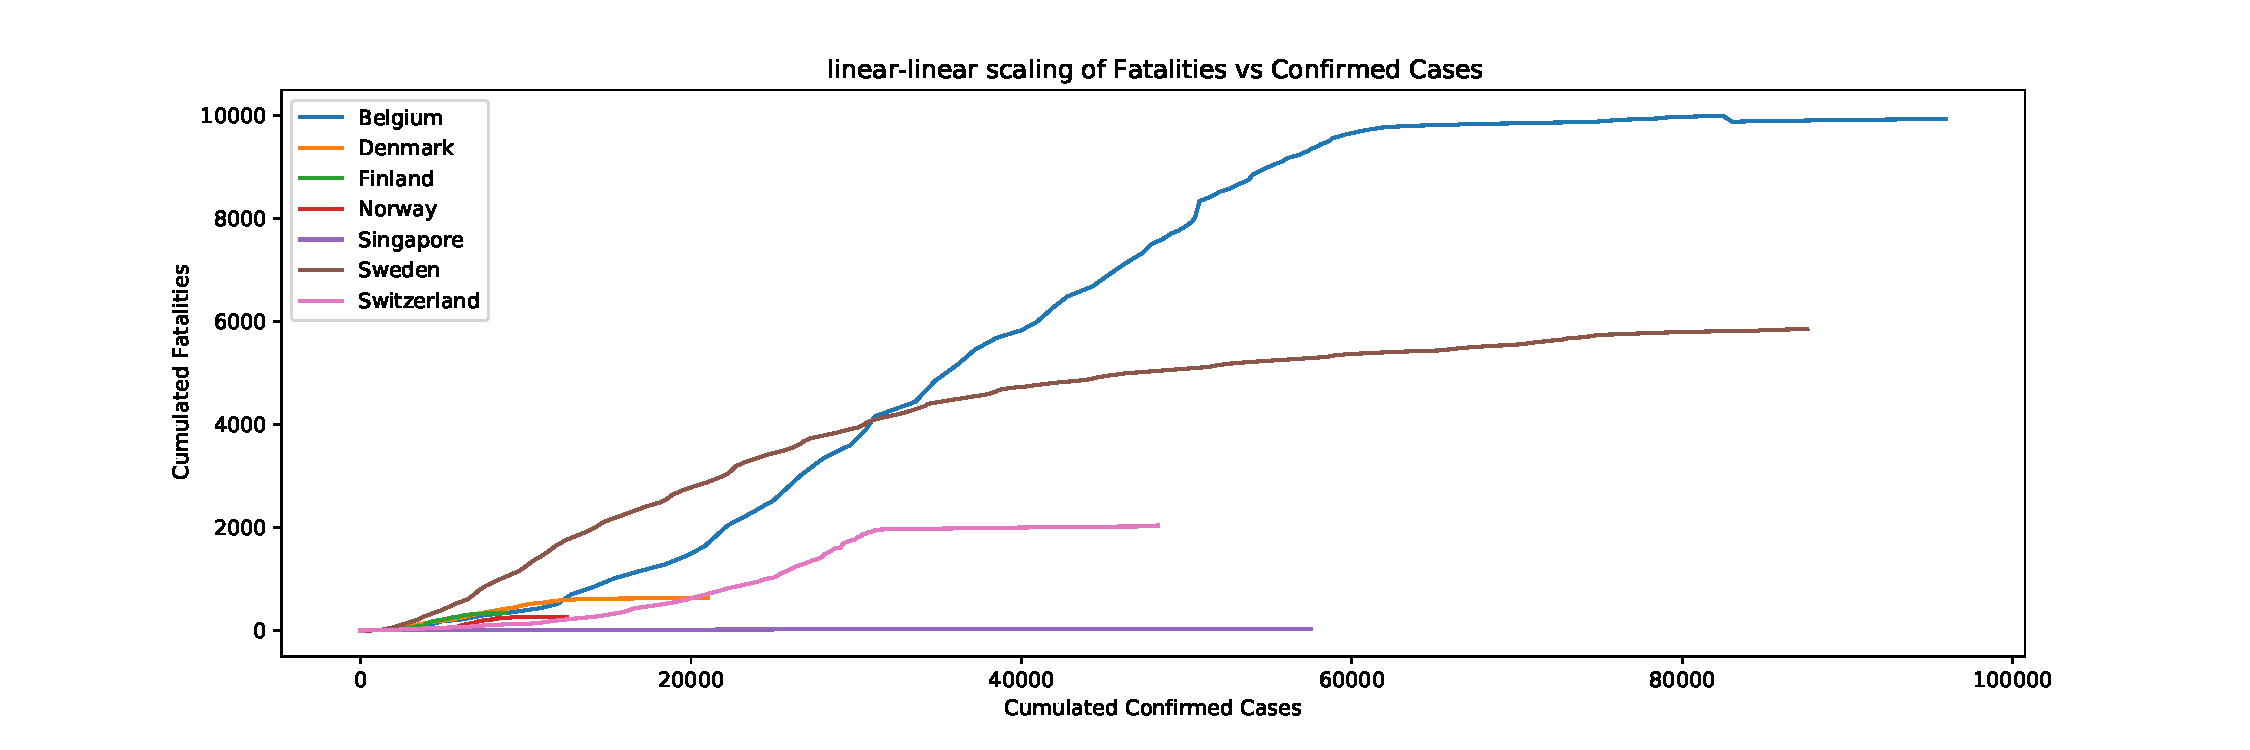
\includegraphics[width=\textwidth]{../figs/parametric_deaths_confirmed_linear.pdf}
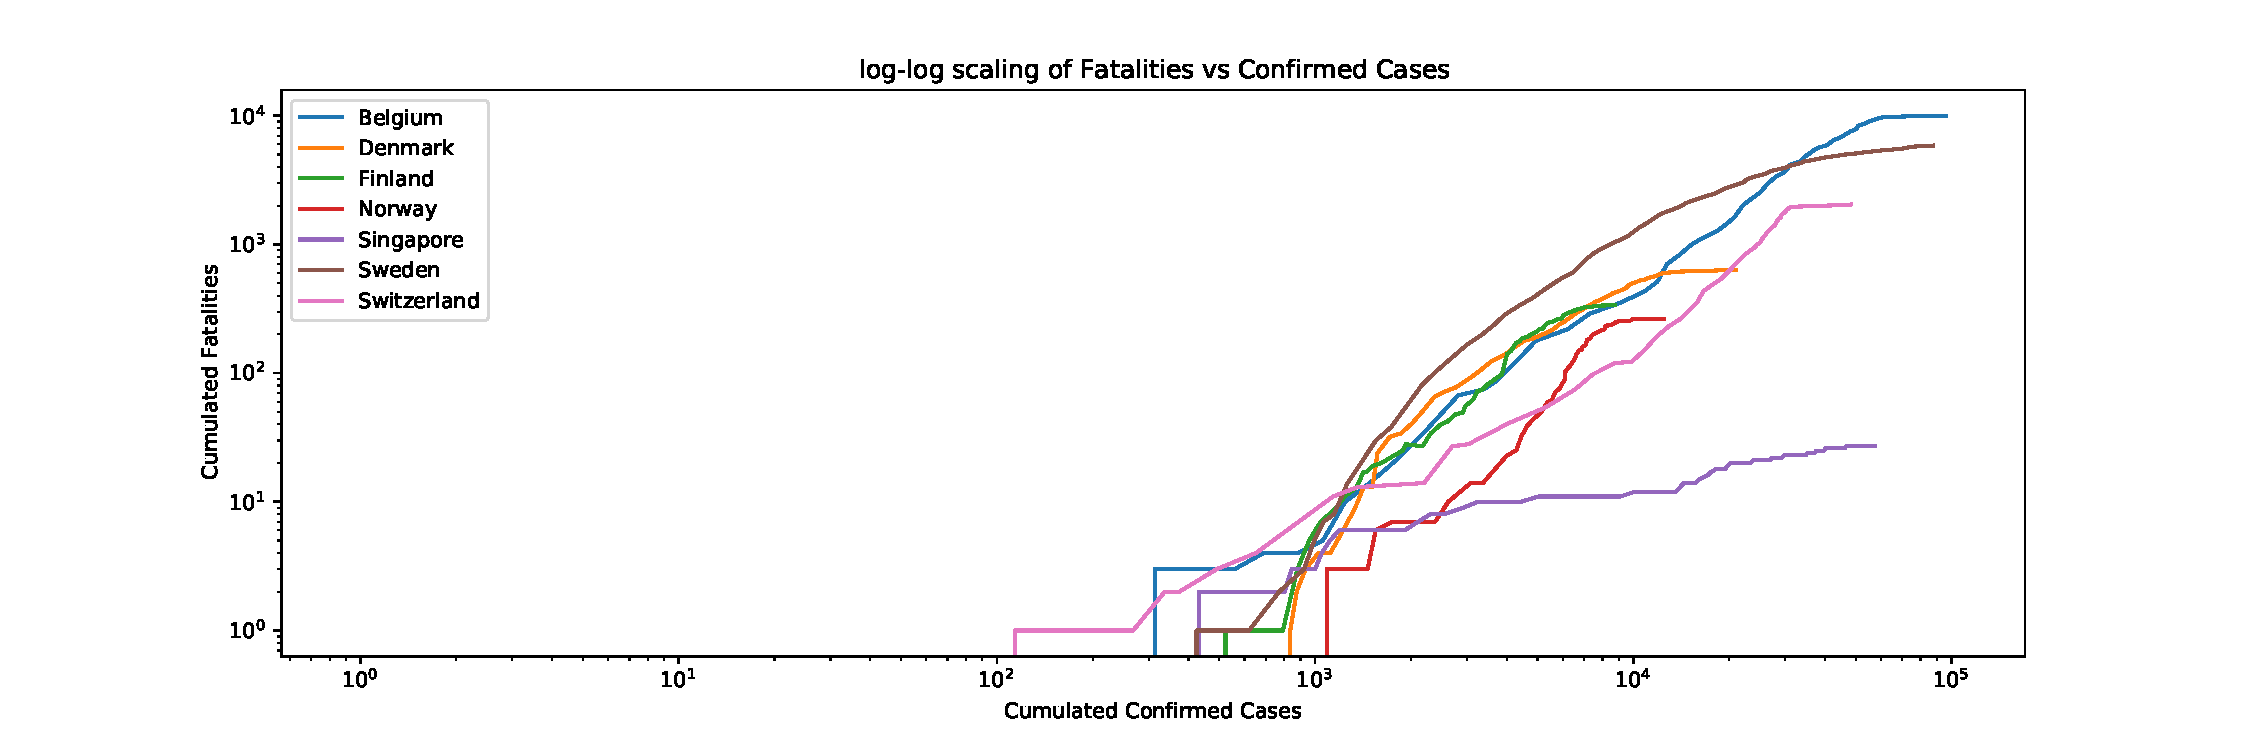
\includegraphics[width=\textwidth]{../figs/parametric_deaths_confirmed_log.pdf}
\end{figure}
\end{frame}
\end{document}

